\section{Krypto Komponenten}

\subsection{NixOS Härtung}

\begin{table}[H]
\centering
\footnotesize
\setlength{\tabcolsep}{4pt}
\renewcommand{\arraystretch}{1.2}
\begin{tabularx}{\linewidth}{@{} >{\RaggedRight}p{2.6cm} >{\RaggedRight}X >{\RaggedRight}X @{}}
\toprule
\textbf{\seqsplit{Härtungsmaßnahme}} & \textbf{Beschreibung} & \textbf{Abgewehrter Angriffsvektor} \\
\midrule
Air-Gap als Standardzustand (Cold-\acp{VM})
  & Das System bootet per NixOS-\emph{specialisation} standardmäßig vollständig air-gapped, ein Online-Modus existiert nur als separater, bewusst zu wählender Boot-Eintrag. Interfaces werden beim Boot heruntergefahren, IPv6 deaktiviert und ausgehender Verkehr per \texttt{nftables} (\texttt{policy drop}, nur Loopback) unterbunden.
  & Remote-Kompromittierung, Exfiltration von Schlüsselmaterial, Command-and-Control. \\
\addlinespace
Festplatten"=verschlüsselung (\acs{LUKS}2)
  & Die Root-Partition ist vollständig verschlüsselt, die Passphrase wird beim Boot abgefragt.
  & Auslesen von Wallet-/Konfigurationsdaten aus gestohlenen Datenträgern oder \ac{VM}-Abbildern (Data-at-Rest). \\
\addlinespace
Kernel-Härtung
  & \texttt{kptr\_restrict}, \texttt{dmesg\_restrict}, \texttt{yama.ptrace\_scope}, deaktiviertes unprivilegiertes eBPF sowie \texttt{protectKernelImage} (kein kexec zur Laufzeit).
  & Lokale Rechteausweitung, Kernel-Informationslecks, Laufzeit-Manipulation des Kernels. \\
\addlinespace
Boot-Integrität
  & Der \texttt{systemd-boot}-Editor ist deaktiviert, sodass Kernel-Parameter am Boot-Menü nicht verändert werden können.
  & Umgehung von Anmeldung bzw. Init-Prozess bei physischem Zugriff. \\
\addlinespace
Kontrollierter Datenträgerzugriff
  & Automatisches Mounten (\texttt{udisks2}) ist deaktiviert, Wechselmedien werden ausschließlich manuell eingebunden.
  & Automatisches Einbinden manipulierter \ac{USB}-Medien. \\
\addlinespace
Reproduzier"=barkeit
  & Passwörter liegen ausschließlich als Hash vor, die Konfiguration ist deklarativ und über einen gepinnten Flake reproduzierbar.
  & Konfigurationsdrift, Klartext-Credentials in der Versionskontrolle. \\
\bottomrule
\end{tabularx}
\caption{Deklarative NixOS-Härtung der Schlüsselhalter-\acp{VM}}
\label{tab:nixos_hardening}
\end{table}


\subsection{PSBT}

\begin{table}[H]
\centering
\footnotesize
\renewcommand{\arraystretch}{1.3}
\begin{tabularx}{\linewidth}{@{} >{\ttfamily\RaggedRight}p{5.0cm} >{\RaggedRight}X @{}}
\toprule
\textbf{\normalfont Status} & \textbf{Beschreibung} \\
\midrule
INTENT\_CREATED & Eingang der \ac{TX}-Anfrage an der \ac{API}-Schnittstelle. \\
\addlinespace
PSBT\_CREATED/PSBT\_FAILED & Nach Erstellung durch den TX-Builder-Microservice über Bitcoin Core. \\
\addlinespace
OPA\_APPROVED/OPA\_REJECTED & Nach der Entscheidung durch den \ac{OPA} (Hot-Wallet). \\
\addlinespace
SIGNED/SIGNING\_FAILED & Nach Signierung auf der \ac{VM} von Key~A. \\
\addlinespace
FINALIZED/FINALIZE\_FAILED & Nach Finalisierung der Hot-\ac{PSBT} zu einer Roh-\ac{TX} über Bitcoin Core (\texttt{finalizepsbt}). \\
\addlinespace
WAITING\_HUMAN & Nach Teilsignierung mit 1/3 Unterschriften, warten auf manuelle Freigabe in der Cold-Wallet-Architektur. \\
\addlinespace
COLD\_STARTED & Der Operator hat die für den manuellen Cold-Prozess generierte \ac{PSBT} auf ein Wechselmedium extrahiert. \\
\addlinespace
COLD\_STOPPED & Eine wartende, veraltete Nachbefüllungs-\ac{PSBT} (WAITING\_HUMAN) wurde gestoppt bzw.\ gelöscht. Eine \ac{PSBT} im Status COLD\_STARTED wird nicht in diesen Status versetzt, sondern bleibt ggf. verwaist in COLD\_STARTED. Dies wird vorgenommen, da ggf. mehrere Operatoren gleichzeitig agieren und das System den menschlichen Handlungsspielraum, wenn dieser einmal gestartet wurde, nicht einschränken soll. \\
\addlinespace
BROADCASTED/BROADCAST\_FAILED & Erfolgreiches bzw.\ fehlgeschlagenes Broadcasting der \ac{TX} über Bitcoin Core (\texttt{sendrawtransaction}). \\
\bottomrule
\end{tabularx}
\caption{\acs{PSBT}-Lebenszyklus und Statusübergänge}
\label{tab:psbt_states}
\end{table}


\subsection{\ac{OPA}}

\begin{table}[H]
  \centering
  \begin{tabular}{@{}l p{7.5cm}@{}}
    \toprule
    \textbf{Policy} & \textbf{Bedingung / Limit} \\
    \midrule
    Pflichtparameter vorhanden (Nicht Null)
      & \texttt{id}, \texttt{psbt}, \texttt{hash}, \texttt{\seqsplit{target\_address}},
        \texttt{\seqsplit{source\_address}}, \texttt{\seqsplit{Wallet\_Typ}} (Voraussetzung für die nachfolgenden Regeln) \\
    \addlinespace
    Netzwerk                & nur \texttt{regtest} \\
    \texttt{amount\_sats}   & $0 < x \le 5\,000\,000$ \\
    \texttt{fee\_sats}      & $\le 20\,000$ \\
    \texttt{fee\_rate}      & $20 \le x \le 100$ sat/vB \\
    \addlinespace
    \texttt{\seqsplit{amount\_sats spent\_today}}
      & $\le 30\,000\,000$ pro Tag (\texttt{\seqsplit{max\_daily\_sats}}, nur Zahlungen, ohne interne Swaps) \\
    \bottomrule
  \end{tabular}
  \caption{\acs{OPA}-Policy zur \acs{PSBT}-Bestätigung (Hot-Wallet)}
  \label{tab:opa_hot}
\end{table}


\subsection{\ac{PCR}}

\begin{figure}[htbp] 
    \centering
    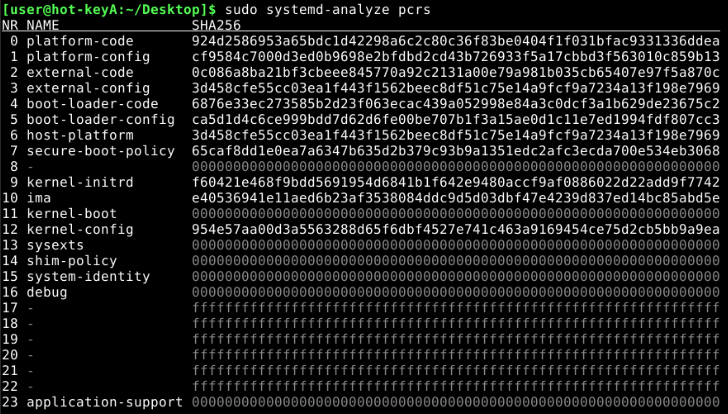
\includegraphics[width=1.0\textwidth]{Doku/Abbildungen/PCR_check.png}
    \caption{Log aus der \acs{PCR}-Abfrage. Quelle: Eigene Bildschirmaufnahme in NixOS.}
    \label{fig:PCR_belegung}
\end{figure}

\pagebreak
\subsection{Hilfsskripte}
\begingroup
\begin{xltabular}{\linewidth}{@{} >{\ttfamily\RaggedRight}p{4.2cm} l >{\RaggedRight}X @{}}
\toprule
\textbf{\normalfont Skript} & \textbf{System} & \textbf{Zweck / Auslöser} \\
\midrule
\endfirsthead

\multicolumn{3}{c}{\tablename\ \thetable{} -- Fortsetzung} \\
\toprule
\textbf{\normalfont Skript} & \textbf{System} & \textbf{Zweck / Auslöser} \\
\midrule
\endhead

\multicolumn{3}{r}{\textit{Fortsetzung auf nächster Seite}} \\
\endfoot

\endlastfoot

\multicolumn{3}{@{}l}{\textit{Basis-System (Hot-Wallet, \path{scripts/ops/})}}\\
refill\slash psbt\_export.sh & Basis & Wartende Cold-\ac{PSBT} auf das Wechselmedium exportieren (Zustand COLD\_STARTED). \\
refill\slash psbt\_broadcast.sh & Basis & Signierte Cold-\ac{PSBT} vom Medium importieren, finalisieren und über Bitcoin Core broadcasten. \\
setup\slash wallet\_import.sh   & Basis & Cold-\path{wsh}-Deskriptor in Bitcoin Core und PostgreSQL registrieren. \\
setup\slash wgHMAC\_import.sh   & Basis & \ac{HMAC}-Geheimnis und \ac{WG}-Konfiguration vom Medium einspielen. \\
setup\slash wgPeer\_export.sh   & Basis & \ac{WG}-Peer-Konfiguration des Basis-Systems exportieren. \\
setup\slash wg\_setup.sh        & Basis & \ac{WG}-Interface und Kernel-Forwarding einrichten. \\
\midrule
\addlinespace
\multicolumn{3}{@{}l}{\textit{Signierer-\ac{VM} (Key~A, Desktop)}}\\
\addlinespace
wgHMAC\_export.sh & Key~A & \ac{xpub}/öffentliche Deskriptoren, \ac{HMAC}-Geheimnis und \ac{WG}-Konfiguration auf \ac{USB} exportieren. \\
wgPeer\_setup.sh  & Key~A & \ac{WG}-Peer einrichten bzw.\ überschreiben. \\
setup.sh          & Key~A & NixOS der Signierer-\ac{VM} automatisiert installieren. \\
mnt/umnt\slash format-USB.sh & Key~A & Wechselmedium mounten, sicher auswerfen bzw.\ bereinigen. \\
\addlinespace
\multicolumn{3}{@{}l}{\textit{Cold-\acp{VM} (Key~B/C, Desktop, \path{setup/})}}\\
\addlinespace
setup.sh          & Cold & NixOS-Cold-Image automatisiert installieren (LUKS, Flake-Pinning). \\
online.sh         & Cold & Kurzzeitig Online-Modus zur Wallet-Registrierung aktivieren. \\
airgap.sh         & Cold & In den air-gapped Standard zurückschalten. \\
mnt/umnt\slash format-USB.sh & Cold & Wechselmedium mounten, sicher auswerfen bzw.\ bereinigen. \\
\midrule
\addlinespace
\multicolumn{3}{@{}l}{\textit{Evaluierte Hash-Freigabeschicht (verworfen, siehe \ref{sec:alt_hash})}}\\
\addlinespace
psbt\slash psbt-approve.sh   & Koord. & \ac{PSBT} hashen und Hash durch den Koordinator signieren (\path{unappr.<id>.psbt}). \\
auth\slash hash-keyGen.sh    & Koord. & Freigabe-Schlüsselpaar auf der Koordinator-Instanz erzeugen. \\
auth\slash hash-keyStore.sh  & Key~B/C & Public Key der Freigabe auf dem Signer hinterlegen (mit Air-Gap-Prüfung). \\
auth\slash hash-verify.sh    & Key~B/C & Freigabesignatur (\path{approval.json.sig}) vor dem Signieren verifizieren. \\
\caption{Betriebs- und Setup-Skripte je System.} \label{tab:skripte} \\

\end{xltabular}
\endgroup